\begin{problem}
  {Q1(b)}
  Consider a network $G = (V,E)$ with a source $s$, a sink $t$, and a capacity $c_e$ on every edge $e \in E$. \\
  Claim: if $f$ is a maximum $s-t$ flow in $G$, then $f$ either saturates every edge out of $s$ or saturates every edge into $t$. \\
  \textbf{False} \\
  \begin{proof}
  \begin{center}
  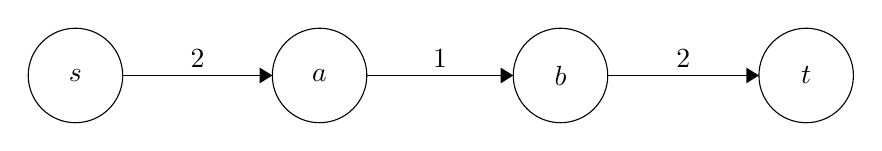
\begin{tikzpicture}[scale=0.2]
  \tikzstyle{every node}+=[inner sep=0pt]
  \draw [black] (8.5,-30.9) circle (3);
  \draw (8.5,-30.9) node {$s$};
  \draw [black] (24,-30.9) circle (3);
  \draw (24,-30.9) node {$a$};
  \draw [black] (39.3,-30.9) circle (3);
  \draw (39.3,-30.9) node {$b$};
  \draw [black] (54.9,-30.9) circle (3);
  \draw (54.9,-30.9) node {$t$};
  \draw [black] (11.5,-30.9) -- (21,-30.9);
  \fill [black] (21,-30.9) -- (20.2,-30.4) -- (20.2,-31.4);
  \draw (16.25,-30.4) node [above] {$2$};
  \draw [black] (27,-30.9) -- (36.3,-30.9);
  \fill [black] (36.3,-30.9) -- (35.5,-30.4) -- (35.5,-31.4);
  \draw (31.65,-30.4) node [above] {$1$};
  \draw [black] (42.3,-30.9) -- (51.9,-30.9);
  \fill [black] (51.9,-30.9) -- (51.1,-30.4) -- (51.1,-31.4);
  \draw (47.1,-30.4) node [above] {$2$};
  \end{tikzpicture}
  \end{center}
  The min cut is $A = \{s,a\}, B = \{b,t\}$. The value of this cut is $1$, which implies the max flow $f = 1$. This does not saturate the edge leaving $s$ or the edge entering $t$. \\
  \end{proof}
\end{problem}
